\chapter{Especificação técnica} \label{cap:metodologia}


\section{Análise de Contexto}

Como visto nos trabalhos correlatos, a utilização de sensores para a detecção de acidentes é necessária, sendo o conjunto composto por acelerômetro e giroscópio o mais comuns para a aplicação. 

O acelerômetro é um dispositivo capaz de medir a aceleração própria de um sistema, dessa forma variações na velocidade impactam nos valores lidos por tal sensor. Os acelerômetros são utilizados para detectar vibrações em sistemas mecânicos, sistemas de navegação de aeronaves, estabilização de voo em drones e ainda para manter a imagem verticalmente nos \textit{smartphones} e \textit{tablets}.

O giroscópio é um dispositivo capaz de manter seu eixo de rotação em uma mesma direção enquanto não houver forças que o perturbem. Quando posicionado em um veículo, o eixo de rotação do giroscópio é mantido independente da direção a qual o veículo está. É utilizado nos sistemas de navegação, substituindo a bússola na navegação marítima e em sistemas de direção autônoma.


\subsection{\textbf{Definições do Sistema}}

O sistema será composto por um \textit{hardware} embarcado fixado na motocicleta, aplicativo para \textit{smartphones} Android e um servidor em nuvem.

Para a detecção dos acidentes, serão utilizados em conjunto o acelerômeto e giroscópio do celular com os sensores de um sistema embarcado no veículo. O sistema embarcado é dotado de sensores semelhantes ao celular e é composto por uma placa microcontrolada e um módulo com o giroscópio e acelerômetro. O \textit{hardware} embarcado e o aplicativo irão comunicar-se através de uma rede \textit{wireless} para troca de informações.

No aplicativo haverá o registro do motorista, armazenando dados de pessoas selecionadas pelo motorista para possíveis avisos, além de informações essenciais para identificação do usuário. O aplicativo será capaz de redirecionar para os relatórios, contendo as áreas com alta probabilidade de risco de acidentes por período e região, além de traçar rotas no Google Maps até a vítima.

O aplicativo irá atualizar a posição do \textit{motoboy} constantemente para que o sistema possa rastreá-lo corretamente em casos emergenciais. Para isso, o aplicativo ficará monitorando majoritariamente o acelerômetro, GPS e possíveis outros sensores do celular.
Quando o aplicativo ou \textit{hardware} realizar a leitura característica de um possível acidente, será disparado um sinal para o serviço em nuvem, este que alertará os outros \textit{motoboys} em um raio de distância de 5km. Os alertados poderão ligar para um serviço de emergência, ir até o local, ou falar com algum parente próximo da vítima ou empregador.

Já o servidor será responsável por receber as informações de localização e irá armazenar estes dados dentro de um banco de dados. Estas informações de rastreio serão apagadas depois de um certo período de tempo pois não há necessidade de manter salvo o trajeto de todos os usuários por longos períodos. Com a latitude e longitude do usuário será possível adquirir informações climáticas, aumentando a capacidade da análise de dados para futuros relatórios.

Quando o servidor receber um sinal de emergência, ele buscará as informações do motorista cadastradas no banco, enviando avisos para todos os usuários próximos da região.

Também serão disponibilizados os dados históricos dos eventos ocorridos em formato tabular, possibilitando a aplicação de filtros para melhor visualização dos relatórios.








\subsubsection{Visão Geral da Arquitetura}

Para tornar o sistema embarcado acessível, o mesmo deve possuir baixo custo, bem como ser pequeno e leve para fácil transporte e instalação. De modo que os critérios sejam cumpridos, faz-se necessário um microcontrolador de baixo custo, em um módulo que já possua comunicação, bem como um conjunto de sensores compactos. Para tal foram selecionados a ESP32 como microcontrolador, esta que possui comunicação wireless, é compacta e de baixo custo, e o módulo MPU-6050, um módulo compacto dotado de acelerômetro e giroscópio capaz de comunicar-se digitalmente.

Desse modo o sistema, em uma visão simplificada, será composto por:

\begin{enumerate}
    \item Aplicativo Android que será utilizado como a interface homem máquina,
além de contribuir com o monitoramento dos sensores e ser responsável
por disparar requisições de avisos para o servidor em nuvem.

    \item \textit{Hardware} embarcado na motocicleta, responsável por monitorar as forças do veículo e auxiliar na detecção dos eventos de interesse.
    
    \item Servidor em nuvem responsável pela recepção, armazenamento e distribuição dos dados adquiridos através de uma interface Web.
    
    \item Interface Web  será responsável por mostrar de forma intuitiva os dados coletados pelo sistema

\end{enumerate}


O sistema terá sua execução divida em 2 partes, a parte local e a parte em nuvem. Na nuvem o sistema será responsável por receber as informações de todos os usuários e ser capaz de tratá-las para poder armazenar ou devolver outra informação para a aplicação. Também é na nuvem que se encontra a página Web, está sendo uma forma de representação dos dados de forma gráfica.

A parte local será o lugar de aquisição de informação e grande parte da interação do usuário com o  aplicativo. Esta área possuirá o embarcado com os sensores acoplados que se comunicarão com o aplicativo Android para a aquisição. A Figura 7 demonstra, de forma resumida, o funcionamento do sistema, na seção de diagramas de blocos será discutido uma versão mais detalhada do sistema.


 \begin{figure}[H]



\begin{center}
     \caption{Diagrama de blocos sucinto }
  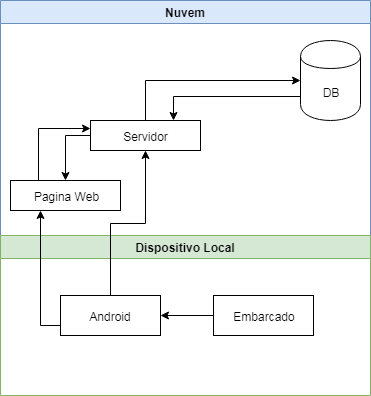
\includegraphics[width=100mm]{images/Cap3/Diagrama_de_blocos.png}
\end{center}
Fonte: Os autores

  
\end{figure}

    

\subsubsection{Funcionamento}

O sistema contará com um aplicativo Android capaz de realizar cadastro de informações sobre o usuário para identificação e rastreio, juntamente serão utilizado os sensores disponíveis no celular para o monitoramento, qualquer variação muito elevada será disparada uma requisição HTTP para o servidor. Os demais aplicativos da proximidade serão alertados do incidente. Com isto poderão visualizar informações essenciais sobre o usuário acidentado podendo se deslocar até o local e efetuar chamadas.

No veículo será acoplado um sistema embarcado para auxiliar nas medições com sensores e controlador a parte. Quando houver alguma variação brusca, o embarcado emitirá um alerta via Bluetooth para o aplicativo que irá emitir uma requisição HTTP para o servidor.

O servidor será responsável pela persistência dos dados recebidos do aplicativo, gerenciamento dos alertas para os dispositivos próximos e disponibilizar informações através de requisições HTTP.


\subsubsection{Atores}

O sistema, como um todo, terá os 2 atores, humano e sistêmico.
O ator humano é responsável, pela interação dentro do aplicativo e navegação dentro da interface Web.

Já o ator sistêmico será todas as mensurações dos sensores além de todas as requisições feitas entre as 4 interfaces já citadas.





\subsubsection{Interfaceamento entre as partes}

O sistema terá como interfaceamento entre as partes  protocolos de comunicação HTTP e Bluetooth, toda a comunicação exterior será feita atráves do protocolo HTTP, já a comunicação local entre o dispositivo e o embarcado será utilizado a tecnologia Bluetooth, a Figura 8 demonstra o interfaceamento do sistema.


O diagrama de blocos apresentado acima possui uma interface de comunicação entre o aplicativo e  o embarcado através da tecnologia Bluetooth onde  enviará as informações necessárias para que o aplicativo android se comunique com o resto dos serviços através do protocolo HTTP através de requisições Web para troca de informações. A página Web também utilizará do mesmo protocolo para sua comunicação.



\begin{figure}[H]

 \caption{Interface do sistema}
\centering
  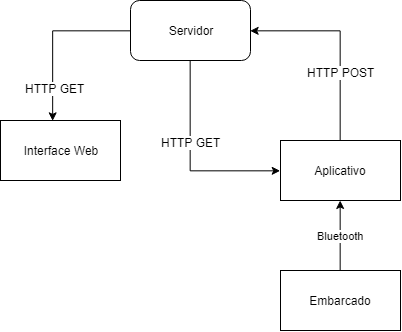
\includegraphics[width=110mm]{images/Cap3/diagrama_funcionamento.png}
            
    
\end{figure}


Fonte: Os autores
    







\subsubsection{Custo do projeto}
A Tabela 2 apresentada os custos para o desenvolvimento do projeto.


\begin{table}[H]
\caption{Custo do projeto}

\begin{adjustbox}{width=80mm,center}


\begin{tabular}{llrr}

\toprule
        Item &  Quantidade &   Custo \\
\midrule
     Servidor &         1.0 &    35.0 \\
       ESP32 &         1.0 &    35.0 \\
   MPU-6050 &         1.0 &    18.5 \\
     CELULAR &         1.0 &   300.0 \\
     NOTEBOOK &         2.0 &  3000.0 \\
 CAIXA PLÁTICA PRETA &         1.0 &    30.0 \\
      LM2596 &         1.0 &    12.9 \\
        Total &           3443.5 \\
\bottomrule
\end{tabular}
    
\end{adjustbox}
\end{table}



\subsection{\textbf{Condições Restritivas}}
\subsubsection{Custos}

O custo estimado para que os usuários utilizem o sistema será de aproximadamente de R\$130, este valor inclui o preço da ESP32 juntamente com o modulo MPU-6050, LM2596 para a alimentação do sistema sem necessidade de uma bateria externa e a caixa plástica para proteção de impacto.


\subsubsection{Recursos}

\begin{enumerate}
    \item Celular Android 5.0 ou superior  e deve conter todos os sensores necessário inclusos no aparelho para que todos os módulos do sistema operem corretamente.  \cite{Android}.
    \item Placa embarcada ESP-32 sendo escolhida por possuir comunicação Bluetooth integrada, é compacta, veloz e de baixo consumo. \cite{Esp32}.
    \item Modulo Acelerômetro MPU-6050 \cite{MPU6050}.
    \item Servidor em nuvem para a realização dos testes do sistema, as configurações do servidor utilizado são de  1GB de memoria RAM, 40GB de armazenamento SSD, Processador Intel Xeon CPU E5-2630 v4 @ 2x 2.2GHz com sistema operacional Ubuntu 18.04 bionic.
    \item Regulador de tensão Step-down (Dc -Dc) LM2596 para ser utilizado na energização do componente embarcado, sendo ligado diretamente na bateria da moto.\cite{StepDown}
\end{enumerate}


\subsubsection{Ambientais}
O \textit{smartphone} é sujeito às condições climáticas, podendo sofrer problemas na comunicação \textit{wireless} com o sistema embarcado e o servidor. O \textit{smartphone} pode não possuir resistência a água, causando possíveis danos ao aparelho conforme exposição. O sistema embarcado é resistente à chuva sendo capaz de suportar respingos de água porém, não é previsto que o mesmo permaneça submerso.


\subsubsection{Físicas e tecnológicas}
O sistema é restritivo aos seguintes itens:
\begin{enumerate}
    \item Modelo do \textit{smartphone} utilizado, limitndo-se a sua versão do sistema operacional sendo necessário possuir no minimo a versão 5.0 (Lolipop) com  API 21.
    O \textit{smartphone} deverá conter todos os sensores necessários no seu \textit{hardware} para a utlização do aplicativo.
    \item Duração da bateria do \textit{smartphone} com no minimo 3000mAh considerando que o celular utlize em média 125mA/h em seu funcionamento durante 24h.
    \item Dependência de rede móvel possuindo no minimo a técnologia 3G para a comunicação estável entre os serviços hospeados na nuvem.
\end{enumerate}

\subsubsection{Energização}

O sistema será dependente da utilização da bateria do celular. Para testes o \textit{hardware} embarcado será dependente de uma bateria, entretanto em cenário real o mesmo utiliza-se da alimentação do veículo.


\subsubsection{Interferências devido ao meio}

A aquisição de dados não deverá sofrer grandes interferências, entretanto as comunicações podem ser comprometidas. A grande presença de ruído eletromagnético, bem como a presença de diversas \textit{redes wireless} no meio podem atrapalhar ou mesmo anular a comunicação entre os dispositivos.

\subsection{\textbf{Benefícios e Impactos}}

\subsubsection{Econômicos}
O aplicativo é destinado à redução do tempo de primeiros socorros especializado em caso de acidentes, gerando uma diminuição de custos de hospitalares, e diminuição da população de pacientes nas UTIS.
\subsubsection{Operacionais}
O sistema é voltado para a fácil utilização, reduzindo a quantidade de iterações do usuário com o mesmo.

\subsubsection{Estratégicos}
O Objetivo é reduzir o tempo de socorro da vitima de acidentes, reduzindo a probabilidade de fatalidades e sequelas.
\subsubsection{Políticos}


A redução no tempo de espera nos postos de saúde, melhora na qualidade da assistência recebida e rápido tratamento especializado para a condição do paciente é esperada. Longos períodos de espera podem gerar uma superpopulação de pacientes, acarretando maior sofrimento para aqueles que esperam aumentando bem como estresse dos pacientes e dos funcionários de saúde.

É esperada a diminuição dos bloqueios no trânsito devido aos acidentes com uma ação mais rápida do sistema emergencial, reduzindo possíveis engarrafamentos e longas filas.





\subsubsection{Sociais}
Aumenta a interação entre os utilizadores, gerando uma maior proatividade para o atendimento de primeiros socorros.


\section{Análise Funcional e de Requisitos}

\subsection{\textbf{Lista de funcionalidades}}
O sistema possuirá as seguintes funcionalidades:

\begin{enumerate}
    \item Monitoramento da localização do motorista para notificação em casos de acidentes;
    
    \item Mensuração dos sensores presentes no smarphone e  dispositivo embarcado, permitindo a tomada de ações com a detecção de eventos pré-definidos;
    
   \item Informações gerais do trânsito coletado pela aplicação serão disponibilizados em uma página Web responsiva a  \textit{smartphones};
   
   \item Tela de notificações de acidentes ocorridos. Através desta tela o usuário poderá ver informações essênciais sobre o ocorrido e tomar algumas atitudes dentro do aplicativo, como realizar uma ligação para o serviço de emergência ou dirigir até o local.
   
\end{enumerate}


\subsection{\textbf{Comunicação}}
Para a comunicação do sistema serão utilizados os seguinte protocolos de comunicação:

\begin{enumerate}
    \item\textit{Bluetooth Standard} é uma tecnologia de comunicação sem fios e de curta distância entre dispositivos eletrônicos. \cite{heydon2013bluetooth}.
    \item Protocolo HTTP: é um protocolo voltado para enviar e receber informações da Web, geralmente  sendo relacionado com um protocolo cliente e servidor utilizando como forma de comunicação as requisições entre as duas partes, com este protocolo é possível se comunicar entre dispositivos por grandes distâncias\cite{tanenbaum2003redes}.
    
    \item Protocolo I2C: é uma comunicação digital cabeada, utiliza-se de barramento e conceitualmente é definida pelo esquema servidor-cliente (Master slave)\cite{paret1997i2c}
\end{enumerate}
O Modulo MPU-6050 se comunica com a ESP-32 atráves do protocolo I2c onde as informações necessárias serão passadas para o  \textit{smartphone} atráves do Bluetooth. O \textit{smartphone} se comunicará com o serviço em nuvem utilizando o protocolo HTTP.





\subsection{\textbf{Processamento}}


      O sistema embarcado será responsável por obter e analisar os dados do sensor MPU-6050. Utilizando-se da linguagem C/C++, o controlador irá determinar os eventos a partir dos dados adquiridos pelo sensor. Com a determinação dos eventos, a comunicação é realizada via Bluetooth com o \textit{smartphone}.
    
     O dispositivo móvel terá como tecnologia o Android nativo e será responsável por receber os dados dos sensores do celular, tratá-los e verificar as suas variações, para que haja  comunicação o dispositivo ira utilizar rede sem fio como 4G, wifi e Bluetooth enviando sinais para o serviço em nuvem. O aplicativo manterá um canal de comunicação via Bluetooth com o dispositivo embarcado permitindo que a detecção de queda pelo dispositivo embarcado seja tratado pelo aplicativo.
    
     O servidor é desenvolvido em Python e se comunica com um banco Postgres, este baseado em SQL relacional. Todas as informações recebidas são tratadas via Python com auxílio de algumas libraries disponíveis como Pandas, Numpy, Psicopg2, entre outras.



\subsection{\textbf{Interface Homem-Máquina}}


A interface homem máquina será disposto de 7 telas principais para a navegação de usuário.

Para o fluxo de login ou cadastro possuirá os campos necessários para a verificação de login do usuário, contando com as informações de nome e senha demostrada na Figura 13, caso o usuário escolha se cadastrar no aplicativo será aberto uma nova janela contendo os campos necessários para realizar o \textit{logon} no aplicativo, logo após o preenchimento será redirecionado para outra tela contendo campos necessários para realizar contato com algum parentesco a Figura 13 demostra o Fluxo das Telas do aplicativo para a realização do cadastro.




\begin{figure}[H]

 \caption{Fluxo de Telas Inicias}
\begin{center}
  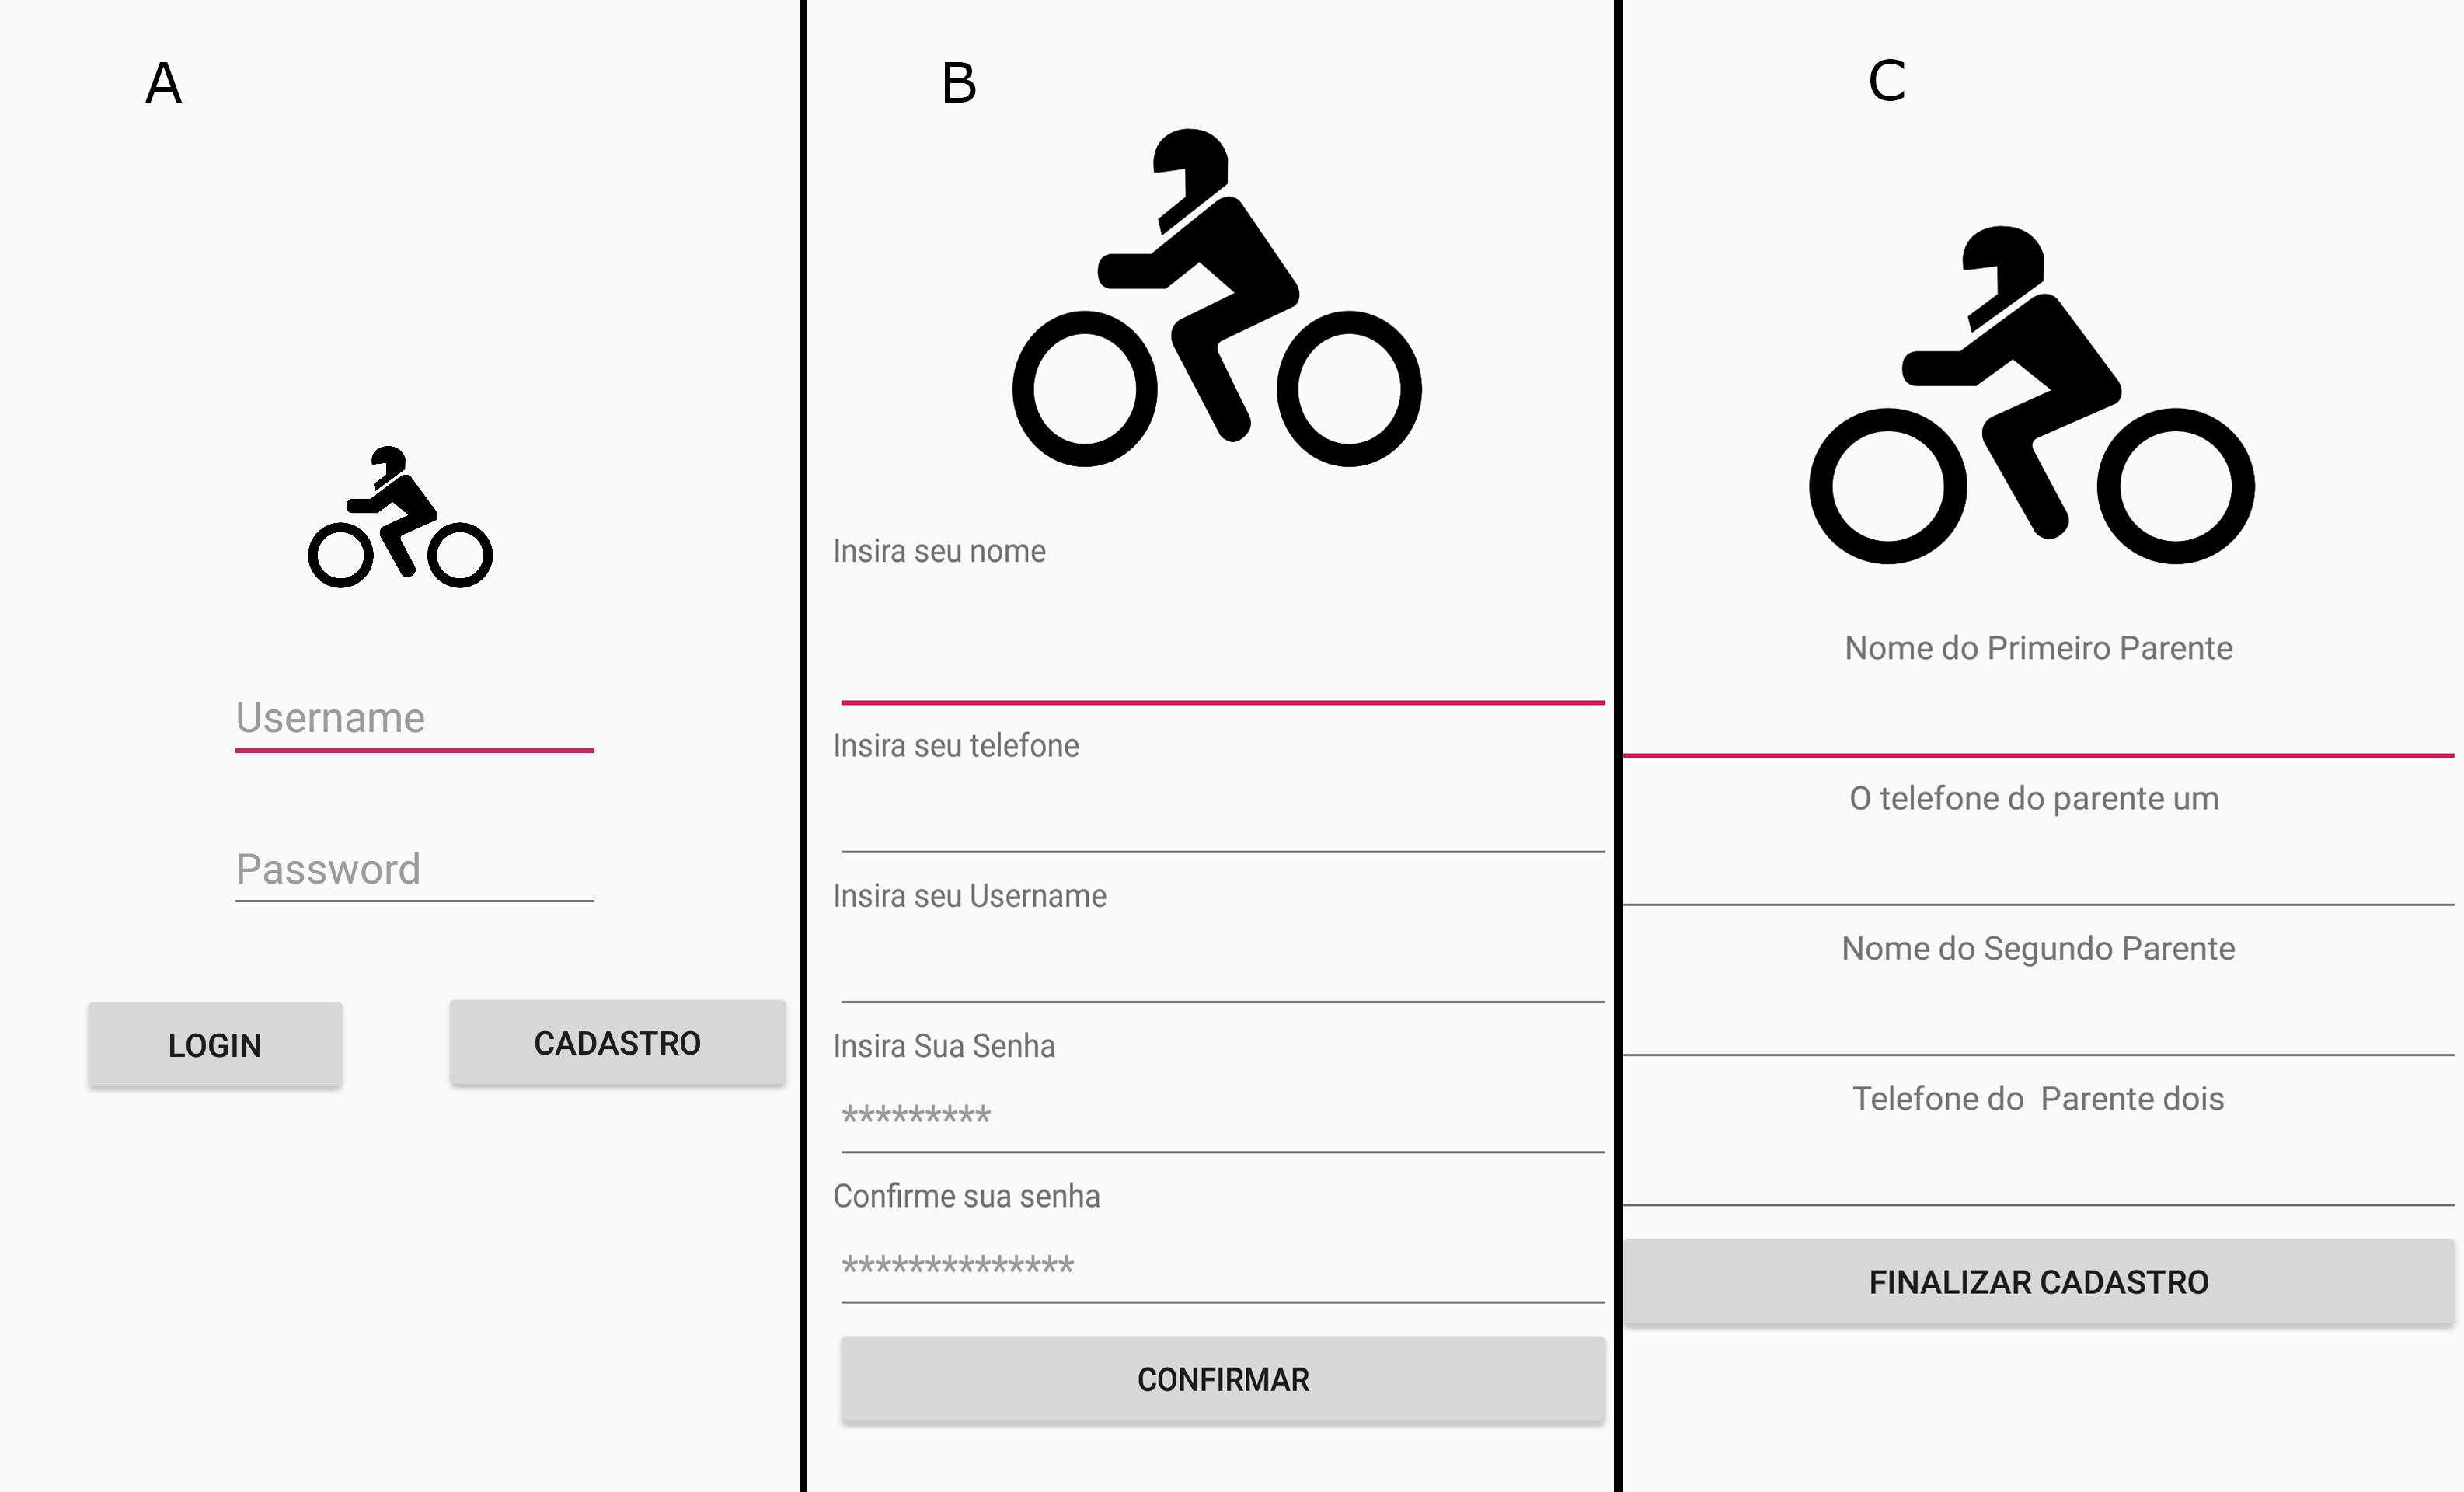
\includegraphics[width=150mm]{images/Cap3/Sequencia-Login.png}
    \end{center}
      Fonte: Os autores
\end{figure}

   

Após o \textit{logon} o usuário será direcionado para a área logada do aplicativo sendo capaz de verificar os avisos recebidos pelo servidor, e poderá ter acesso às informações das vítimas sendo possível tomar algumas ações como ligar para o órgão de saúde publica , ligar para algum parentesco, ou traçar a rota via Google Maps até a vítima a Figura 14 demostra o fluxo de acesso as informações das notificações.

\begin{figure}[H]

 \caption{Fluxo de Notificação}
\begin{center}
  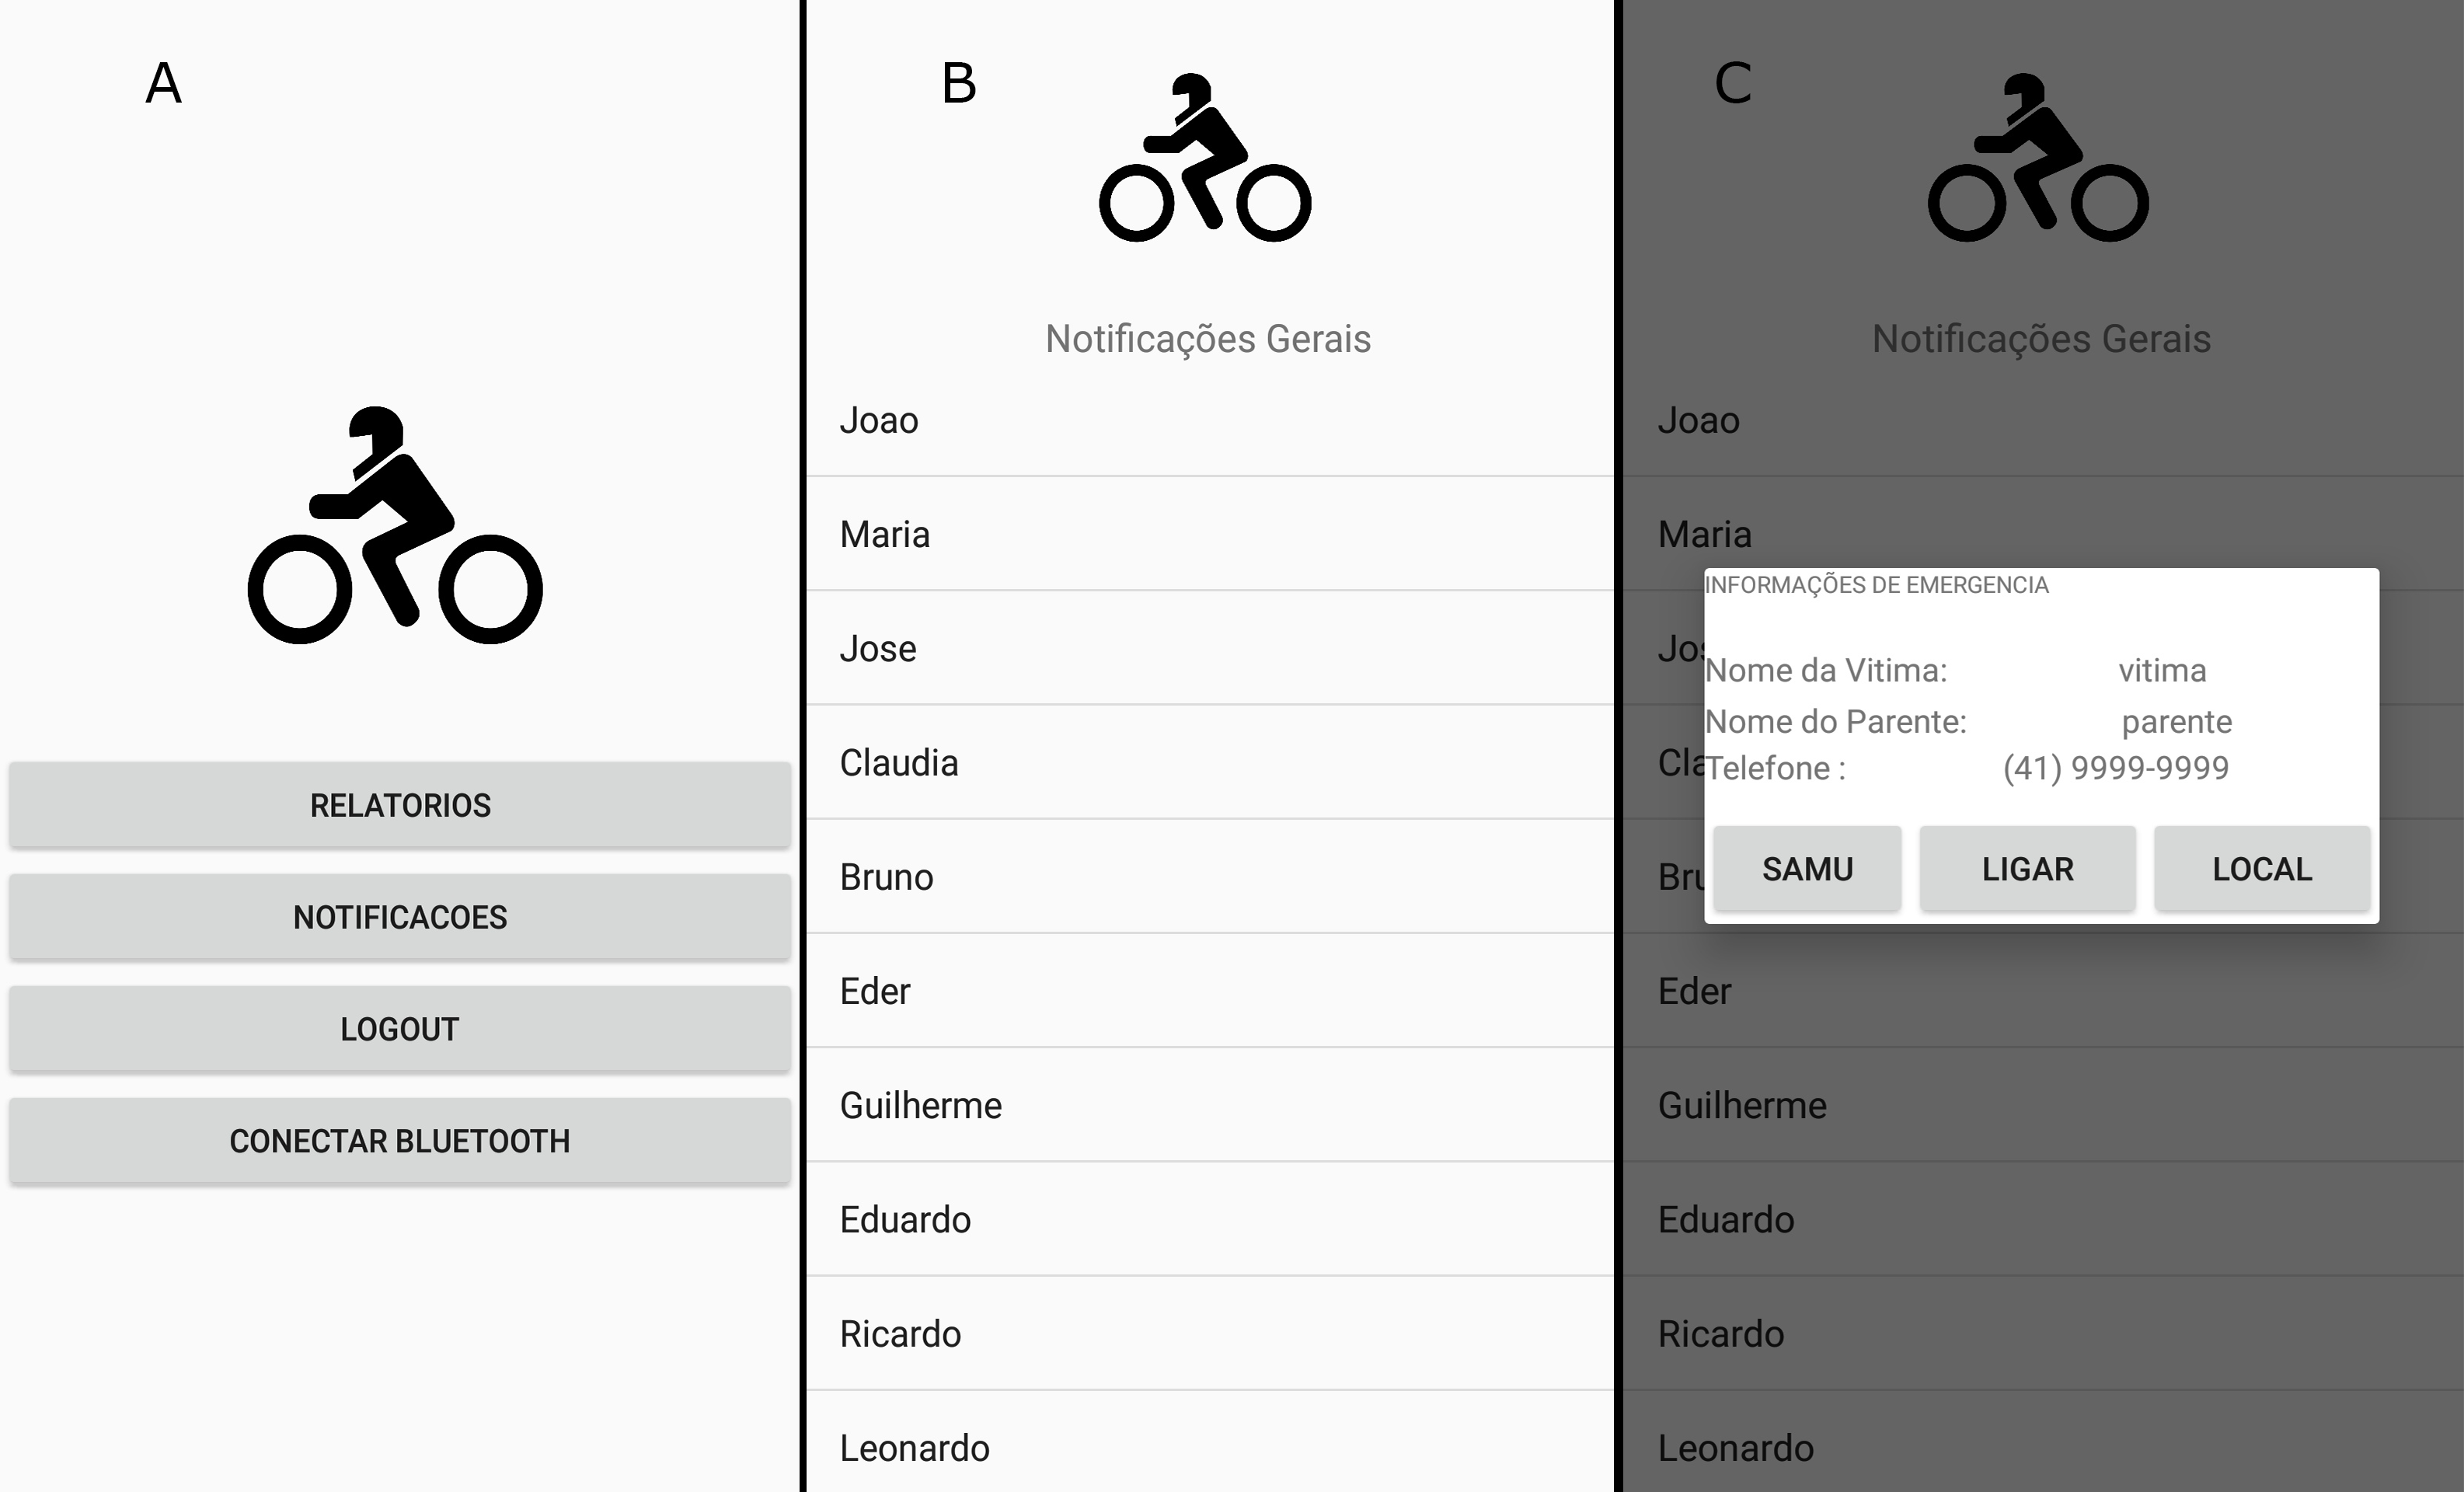
\includegraphics[width=150mm]{images/Cap3/sequencia_notificacao.png}
    \end{center}
     Fonte: Os autores
\end{figure}


E para finalizar o usuário poderá interagir com o dashboard onde conterá as informações gerais dos dados recebidos pelo aplicativo a Figura 15 mostra o fluxo de telas para o \textit{dashboard}.

\begin{figure}[H]

 \caption{Fluxo de Notificação}
\begin{center}
  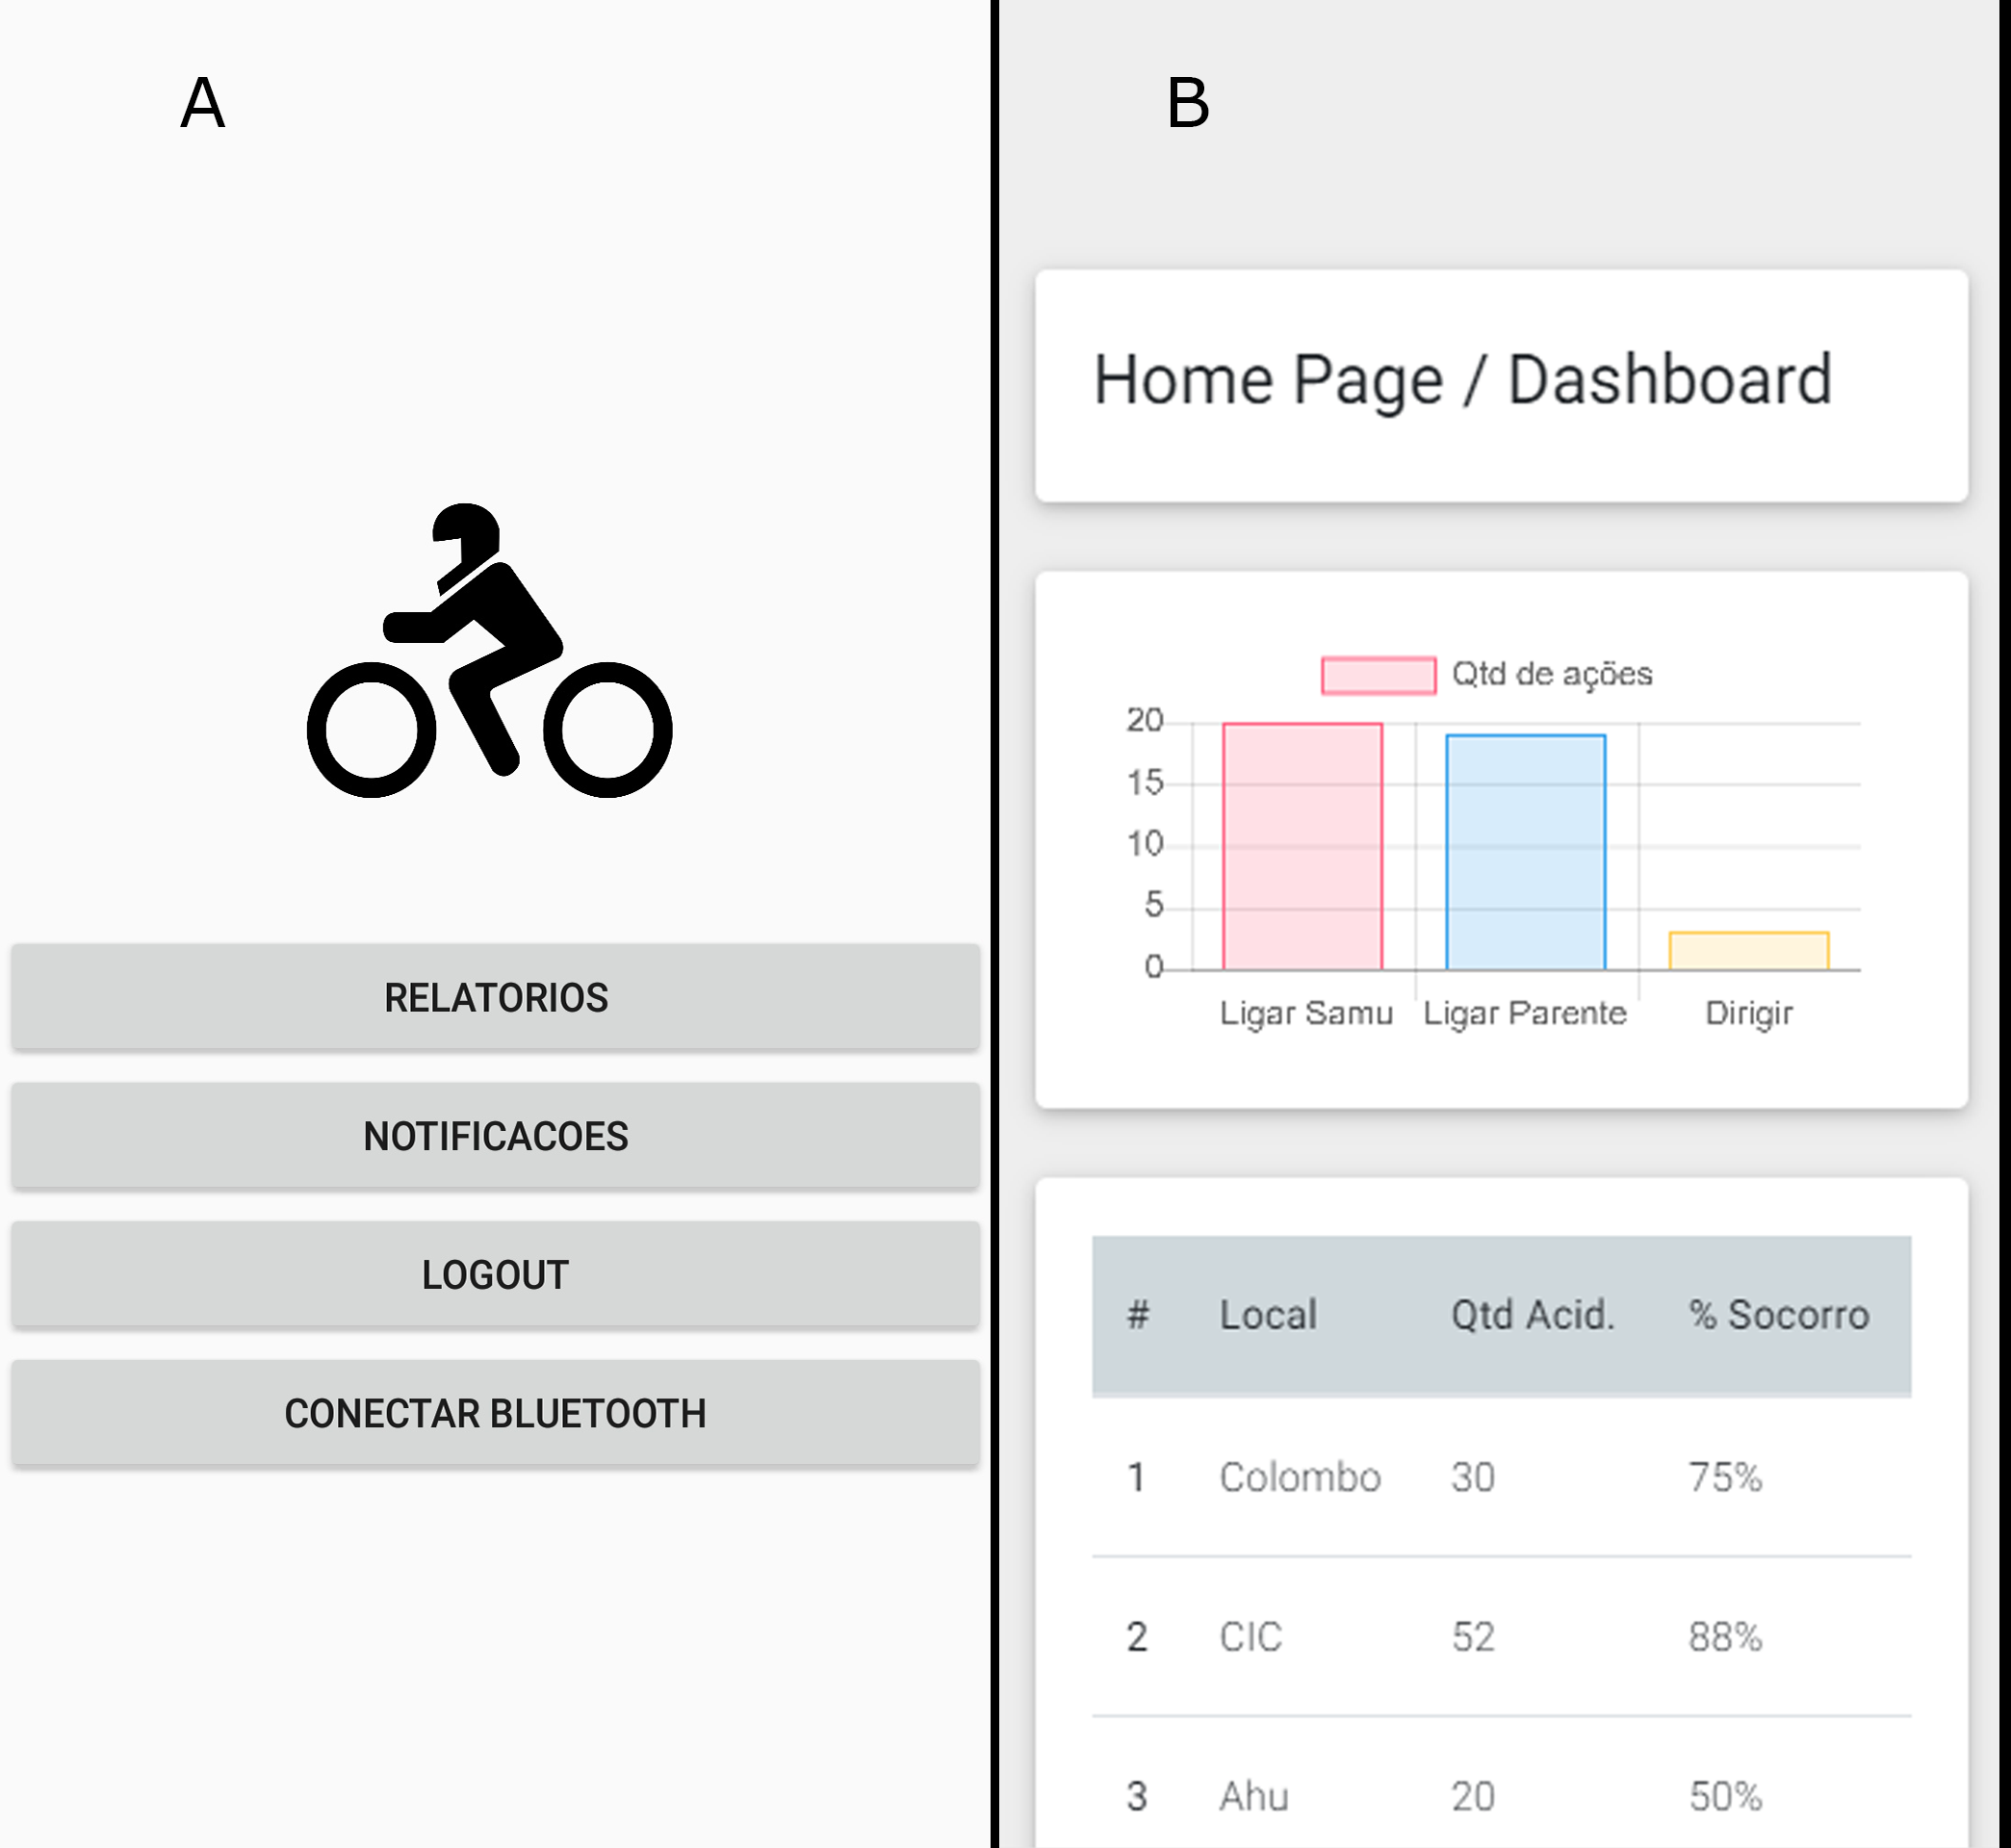
\includegraphics[width=100mm]{images/Cap3/Sequencia_dash.png}
    \end{center}
     Fonte: Os autores
\end{figure}


    



\subsection{\textbf{Sistemas Controlados Automaticamente}}
Para o sistema todas as 4 interface possuem uma parte automatizada, sendo elas:

\begin{enumerate}
    \item Para o dispositivo embarcado toda parte de monitoramento do sensor e comunicação com o dispositivo móvel será feita de forma autônoma;
    
    \item No aplicativo Android o monitoramento dos sensores e comunicação com o servidor e sistema embarcado é feita de forma automática;
    
    \item No servidor todas as tratativas de dados, armazenamento e aquisição dos dados será feita de forma automática;
    
    \item A plataforma Web será totalmente automática na aquisição e população dos gráficos dentro da página.
    
\end{enumerate}


\subsection{\textbf{Aquisição de dados}}



Os dados serão adquiridos através do sistema embarcado e o dispositivo móvel. Utilizando o MPU-6050, a ESP irá determinar quando houver um acidente, notificando o aplicativo. O MPU ainda conta com um Digital Motion Processor (DMP). O DMP é um chip auxiliar capaz de executar algoritmos complexos de 6 eixos, a utilização do mesmo exclui a necessidade de utilizar um filtro complementar nos dados obtidos uma vez que sua função é tratar os dados internamente sem sobrecarregar outros sistemas. O MPU utiliza da interface I2C para comunicar-se com a ESP, notificando a presença de dados a serem obtidos por meio de uma interrupção.



O sistema do celular utiliza o acelerômetro e giroscópio embutidos no aparelho, com isso é realizado o mesmo procedimento descrito para o embarcado, porém o sistema Android ainda irá usar o GPS também nativo do aparelho para localizar o usuário.




\subsection{\textbf{Atuação}}

O sistema atuarará como ponte de prestação de primeiros socorros para os utilizadores, tendo como foco a redução do tempo resposta aos acidentes no trânsito dos motociclistas.


\section{Análise da Arquitetura do Sistema}
\subsection{\textbf{Hardware}}
\subsubsection{Diagrama de Blocos}

O \textit{hardware} é composto por dois módulos, sendo eles a ESP-32 e MPU-6050. A aquisição de dados é realizado pelo MPU, estes dados são interpretados pela ESP que determina o tipo de evento realizado pela motocicleta. 


\begin{figure}[H]

    \caption{Diagrama de blocos da comunicação dos modulos no embarcado}
      \begin{center}
          
      
    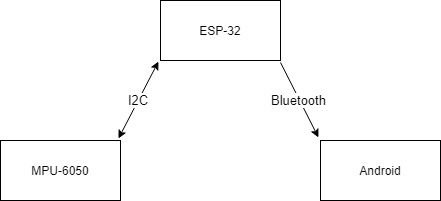
\includegraphics[width=120mm]{images/Cap3/Diagrama_hardware.png}
    \end{center}
         Fonte: Os autores
\end{figure}





Com o diagrama completo é possível notar que toda comunicação será feita em duas partes, sendo uma localmente composta pelo dispositivo Android e sistema embarcado e outra entre a nuvem e o dispositivo Android. A nuvem é composta por toda a parte do servidor e manipulação da página Web.

Na parte local, composta pelo sistema embarcado e aplicativo, ocorrerá uma comunicação via Bluetooth. O sistema embarcado tem a função de enviar um sinal de emergência para o dispositivo somente quando um evento de acidente for detectado. Com a detecção de acidente o aplicativo enviará um sinal para o servidor contendo a localização do usuário.

O servidor irá receber estas informações e, com base na posição recebida do aparelho, listará todos os dispositivo próximos notificando-os.
Os aplicativos mais próximos a região serão notificados, armazenando as informações do usuário acidentado temporariamente. O usuário que receber a notificação no aparelho poderá executar ações reativas à situação.

Todas as informações relevantes e de interesse serão salvas para que sejam populadas em uma página Web. A Figura 17 demostra o diagrama de blocos detalhado do sistema.


\begin{figure}[H]
 
    \caption{Diagrama de blocos Geral}
    \begin{center}
    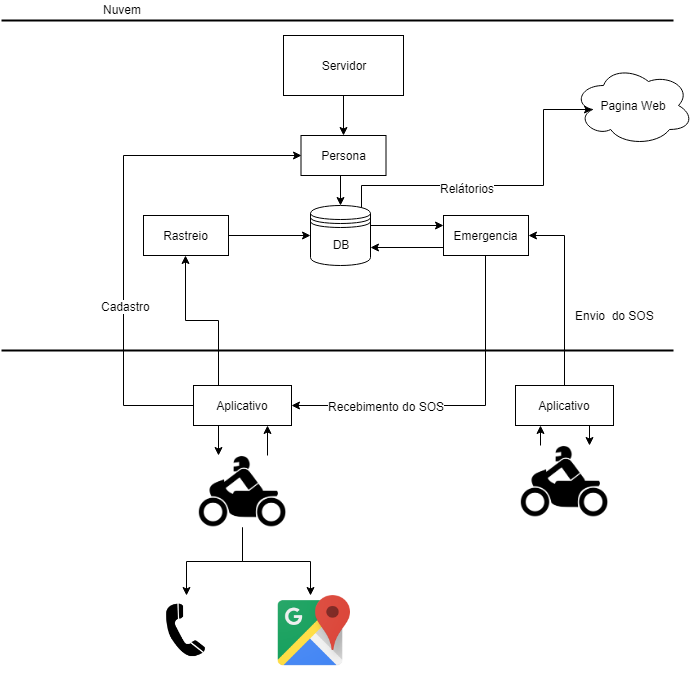
\includegraphics[width=120mm]{images/Cap1/tcc.png}
    \end{center}
       Fonte: Os autores
\end{figure}

  


\subsubsection{Diagrama de Fluxo para \textit{Firmware}}

O \textit{firmware} da ESP é responsável por identificar os eventos de acidentes baseando-se nos dados adquiridos pelo MPU, notificando o aplicativo via \textit{Bluetooth Standard}.

Quando a ESP é alimentada, é realizada a inicialização do módulo MPU e comunicação Bluetooth, permitindo que haja a comunicação I2C com o MPU e o pareamento com o aplicativo. Assim que a inicialização é bem sucedida, o sistema embarcado aguarda pelo pareamento do Bluetooth. Caso ocorra algum problema na inicialização de um dos componentes, o \textit{firmware} fica no estado de inicialização.

Enquanto a Bluetooth estiver conectado, o ESP realiza a comunicação com o MPU, obtendo as leituras de seus sensores e analisando os dados para detectar possíveis acidentes. Tendo uma identificação de acidente, a ESP notifica o aplicativo via Bluetooth.
O fluxo de operação é demonstrado na Figura 18.  

\begin{figure}[H]

 \caption{Diagrama de firmware}
\begin{center}
  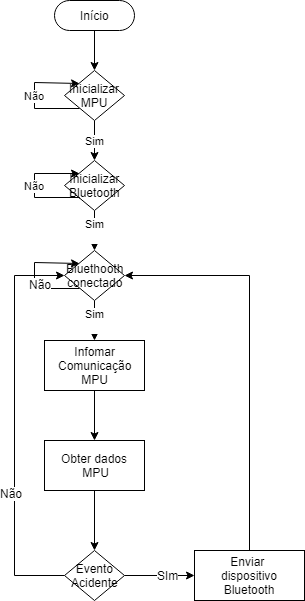
\includegraphics[width=100mm]{images/Cap3/diagrama_firmware.png}
  \end{center}
      Fonte: Os autores   
\end{figure}





\subsection{\textbf{Software}}
\subsubsection{DER/MER}


O banco relacional terá ao todo 5 tabelas. Possuindo uma tabela de usuários, encarregada de armazenar as informações sobre o utilizador, uma tabela de atualização de posição sendo responsável por armazenar o status de deslocamento do \textit{motoboy} para sua localização.

Possuirá uma tabela de parente, armazenando as informações de contatos pessoais de cada usuário, as tabelas relacionais sendo uma tabela de notificação responsável por receber o aviso de acidente e com isso cruzar as informações necessárias das outras tabelas para encontrar as informações do usuário acidentado.

Por fim existe uma tabela sem relacionamento sendo responsável por armazenar a posição do acidente, sua data de ocorrência e o clima para que em um dos relatórios do \textit{dashboard} seja detalhado sobre a localização do acidente e como estava o clima na hora do ocorrido. A Figura 19 demostra todo o diagrama de entidade relacionamento do banco.



\begin{figure}[H]

 \caption{Diagrama de entidade e relacionamento}
\begin{center}
  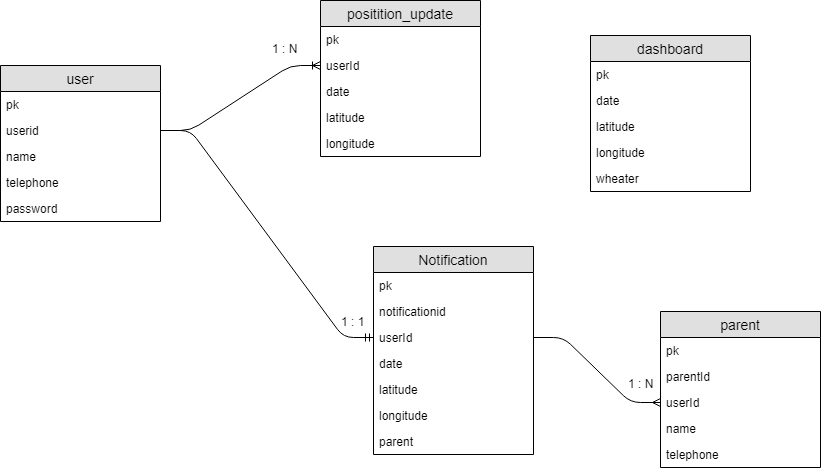
\includegraphics[width=150mm]{images/Cap3/ER.png}
  \end{center}
     Fonte: Os autores 
\end{figure}

   





\subsubsection{\textit{Use Case}}

O diagrama da Figura 20 representa o uso do aplicativo demonstrando o fluxo de ações que o usuário poderá executar. A primeira interação necessária para o uso do aplicativo é a tela de login, a partir dela o usuário poderá tanto cadastrar-se ou entrar em uma conta existente. 
Quando \textit{logado}, o usuário será redirecionado para a area principal do aplicativo. Nesta area o usuário poderá ver as notificações recebidas pelo aplicativo ou ir para a página de \textit{dashboard} onde poderá verificar os relatorios disponibilizados pelo aplicativo.




\begin{figure}[H]

 \caption{Diagrama de Caso de Uso}
\begin{center}
  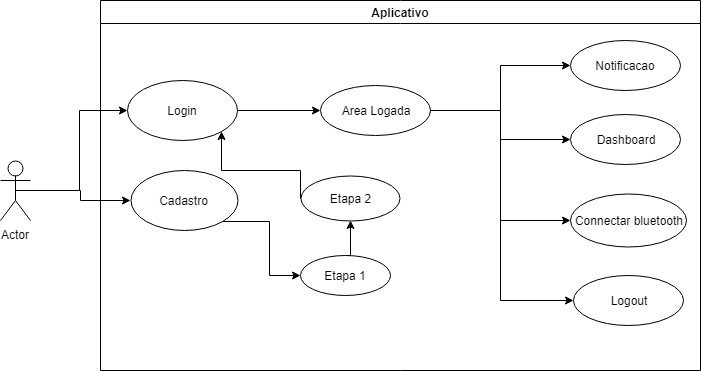
\includegraphics[width=150mm]{images/Cap3/Diagrama_de_Caso_de_Uso.png}
  \end{center}
      Fonte: Os autores
\end{figure}

 




\subsubsection{Diagramas de Sequência}

O diagrama de sequência ou UML é responsável por demonstrar o fluxo do aplicativo conforme a interação do usuário. O UML referente ao aplicativo é detalhado a seguir.

A primeira ação que o usuário deverá tomar dentro do aplicativo é fornecer os dados cadastrais ou, se não tiver cadastro, deverá ser redirecionado para a tela de cadastro do aplicativo. O cadastro é composto de duas etapas com a aquisição da informação necessária para a criação de seu acesso dentro do aplicativo.
Quando o usuário efetua o \textbf{login} corretamente é direcionado para a area principal do aplicativo, também conhecida como “Área Logada”. Neste lugar o usuário poderá executar diversas interações como ser redirecionado para a página Web e verificar as notificações de sinais de emergência. A tela principal também será responsável pela conexão do aparelho com o embarcado.
Com as informações descritas anteriormente, foi criado um diagrama de sequência do aplicativo demonstrado na Figura 21, contendo todo fluxo do usuário juntamente com seus retornos.


\begin{figure}[H]

 \caption{Diagrama de Sequência}
\begin{center}
  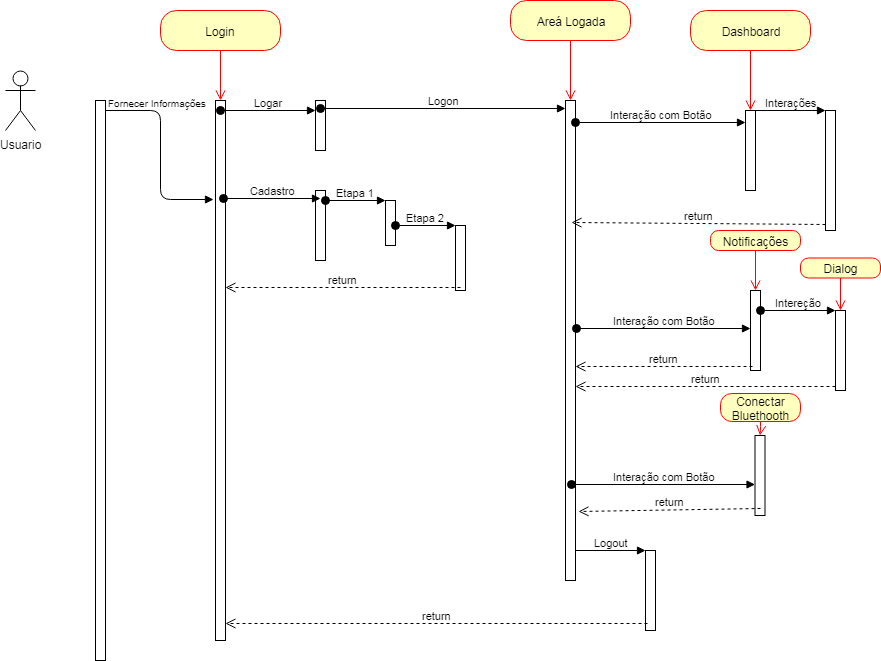
\includegraphics[width=150mm]{images/Cap3/Diagrama_de_Sequencia_Android.png}
  \end{center}
      Fonte: Os autores
    
\end{figure}

 






\subsubsection{Diagramas de Classe}

O diagrama de classe do dispositivo android foi divido em 3 partes para facilitar o entendimento do sistema.
A primeira parte é composta pelas telas do aplicativo. Cada bloco representa o nome da tela e as setas definem o fluxo de comunicação do sistema.

As aplicações que devem ser executadas em \textit{Foreground}, ou serviços que devem ser rodados em primeiro plano dentro do sistema, são os serviços responsáveis pela aquisição dos dados e comunicação entre o celular e o dispositivo.

Os serviços em primeiro plano dentro do Android não necessitam diretamente da interação do usuário pois também são um método de criação de serviço em que o sistema operacional consiga gerenciá-lo mesmo após o fechamento da aplicação principal.

Os serviços em \textit{background} são responsáveis por fazer a comunicação com o servidor. Este serviço tem por função enviar e receber as informações para a nuvem. A Figura 22 representa o diagrama de classes da aplicação Android.



\begin{figure}[H]

 \caption{Diagrama de classe Android}
\begin{center}
  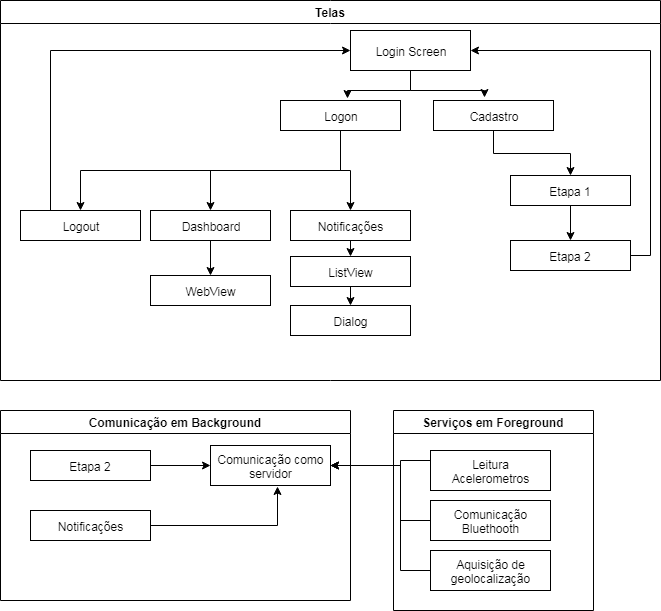
\includegraphics[width=150mm]{images/Cap3/Diagrama_de_Classes-Android.png}
  \end{center}
   Fonte: Os autores
    
\end{figure}

    


O servidor possuirá uma classe assíncrona principal em execução que será o HTTPServer. Esta classe será responsável por gerir todo o tráfego de requisição, adquirindo as informações necessárias para retornar corretamente o que foi solicitado.

As classes criadas terão o papel de tratar os dados recebidos, adquirir e modelar os dados armazenados do banco de dados para gerar o retorno correto conforme as requisições realizadas.

Para a fácil visualização do diagrama completo foram reaproveitados os \textit{sprites} do banco, de forma que o diagrama fosse montado de maneira mais intuitiva de se visualizar. A Figura 23 demonstra o diagrama do Servidor.


\begin{figure}[H]

 \caption{Diagrama de classe Servidor}
\begin{center}
  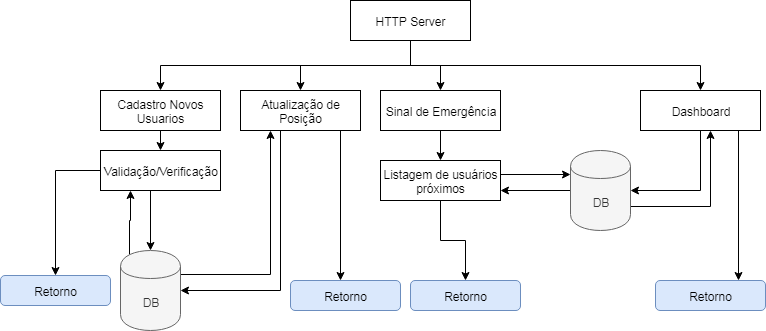
\includegraphics[width=150mm]{images/Cap3/Diagram_de_Classes_Servidor.png}
  \end{center}
    Fonte: Os autores
\end{figure}

De todas as partes do sistema a página Web torna-se a mais simples em termos de classes, pois possui as funções de manipulação do DOM, ou seja, de navegação do usuário dentro da página e realizar as requisições assíncronas para a aquisição e inserção dos dados nos gráficos existentes dentro da página Web. A Figura 24 demonstra os componentes necessários para o funcionamento da página. 


\begin{figure}[H]

 \caption{Diagrama de classe da pagina Web}
 \begin{center}
  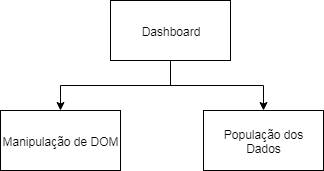
\includegraphics[width=100mm]{images/Cap3/Diagrama_de_Classes_Pagina_Web.png}
  \end{center}
    Fonte: Os autores 
\end{figure}


\subsubsection{Diagrama de Funcionamento FCM}

As notificações serão feitas automaticamente utilizando o serviço da Google chamado \textit{Firebase Clound Messaging} (FCM), a partir dele será disparado avisos entre os dispositivos conectados ao aplicativo.
Quando o \textit{motoboy} se acidentar será enviado um aviso de forma automática para o servidor, quando recebido esta informação o servidor irá pegar a lista dos usuários ativos e irá calcular a distância de cada usuário em relação ao acidente, após a seleção dos usuários que irão receber a notificação será criado um grupo de pessoas que será disparado o envio da mensagem utilizando a aplicação da Google.

Será necessário fazer o filtro de proximidade pois a quantidade máxima de pessoas que podem receber a mensagem por grupo é limitado a 1000 usuários por grupo a Figura 25 demostra o fluxo de funcionamento do Firebase Clound Messagin.

    


\begin{figure}[H]

 \caption{Diagrama de classe da pagina Web}
 \begin{center}
  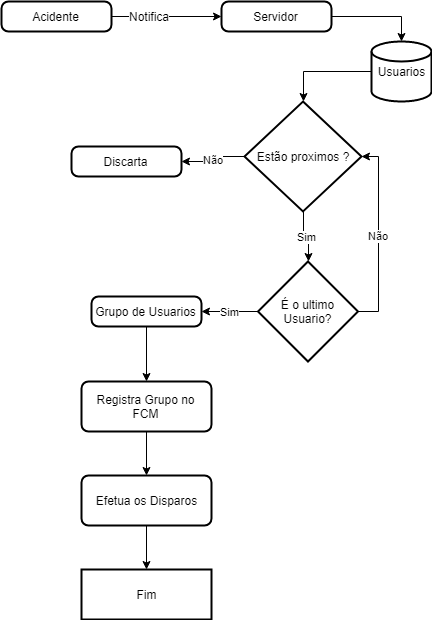
\includegraphics[width=100mm]{images/Cap3/Fluxo_Firebase.png}
  \end{center}
    Fonte: Os autores 
\end{figure}